% !Mode:: "TeX:UTF-8"
% !TEX program  = xelatex
\documentclass{sdureport}

% no head line or foot line
%\pagestyle{empty}

% just for filling a few pages
\usepackage{blindtext}

% initialize the variable texts
\sduCollege{计算机科学与技术}
\sduCourse{社交媒体与舆情分析}
\sduSdudentId{201605130115}
\sduName{崔晨}
\sduClass{菁英班}
\sduExperimentalTopics{情感分析}
\sduDate{2019年11月1日}
\sduEmail{chentsuei@gmail.com}

\begin{document}
\begin{sduDocument}	

	\section{实验方法介绍}
	
	词袋模型(英语:Bag-of-words model)是个在自然语言处理和信息检索(IR)下被简化的表达模型。此模型下,一段文本(比如一个句子或是一个文档)可以用一个装着这些词的袋子来表示,这种表示方式不考虑文法以及词的顺序。最近词袋模型也被应用在计算机视觉领域。

	\section{实验过程描述}
	
	\subsection{数据处理}
	
	分词、构造词表...
	
	\subsection{模型训练}
	
	分词、构造词表...
	
	\section{结论分析}
	
	\begin{enumerate}
		\item 迭代次数:1868
		\item $\theta$:[-0.0566, 1.4720, 1.5706]
		\item 见:图\ref{L1}
		\item 见:图\ref{b1}
		\item 此学生不被录取的概率:0.6680
	\end{enumerate}
	
	\begin{figure}[H]
		\subfigure[Loss 变化曲线]{
			\label{L1}
			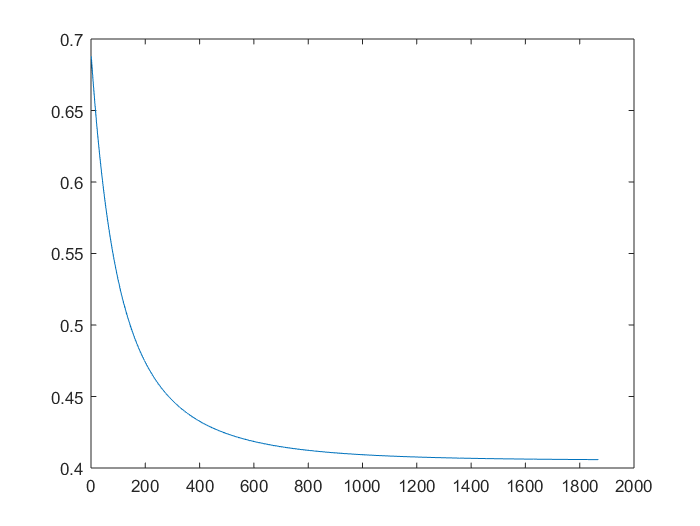
\includegraphics[width=0.45\textwidth]{image/L1.png}}
		\subfigure[Decision Boundary]{
			\label{b1}
			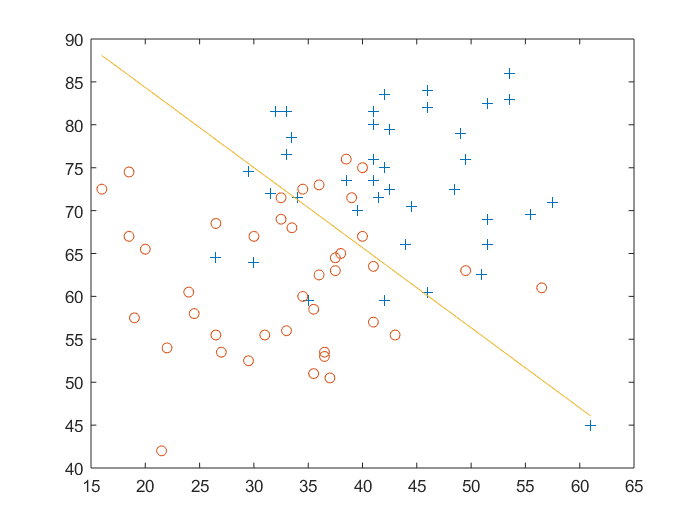
\includegraphics[width=0.45\textwidth]{image/b1.png}}
		\caption{梯度下降法}
	\end{figure}
	\begin{figure}[H]
		\subfigure[Loss 变化曲线]{
			\label{L2}
			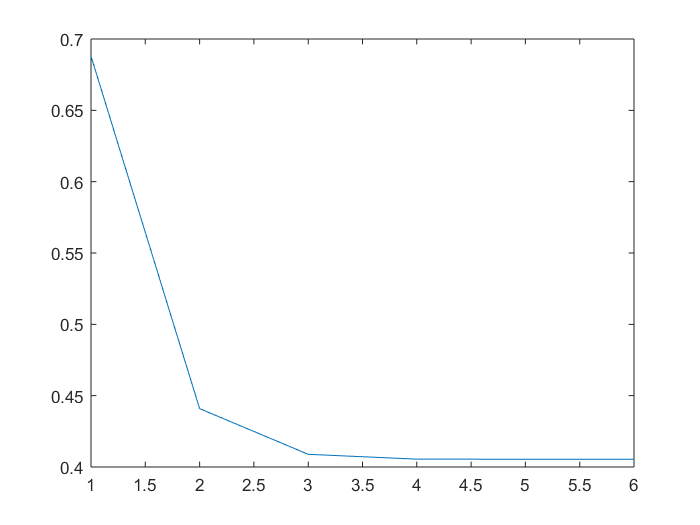
\includegraphics[width=0.45\textwidth]{image/L2.png}}
		\subfigure[Decision Boundary]{
			\label{b2}
			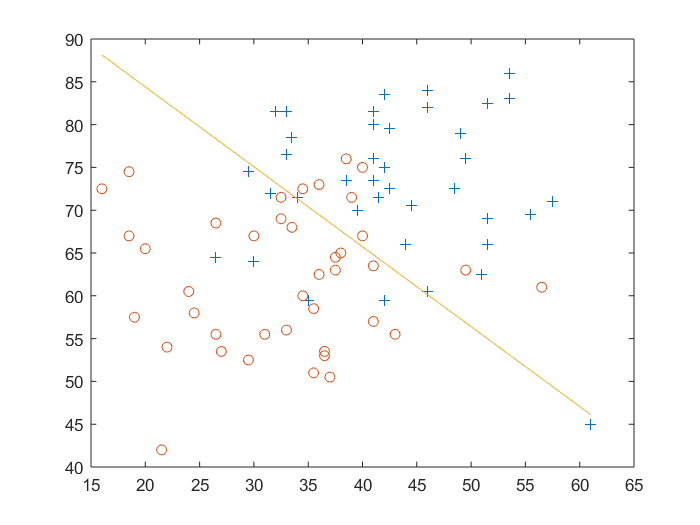
\includegraphics[width=0.45\textwidth]{image/b2.png}}
		\caption{牛顿法}
	\end{figure}
	
	实验结果显示...
	
	\section{结论}
	
	基于朴素贝叶斯的方法...
	

\end{sduDocument}

\begin{lstlisting}[language=python]
print('Hello World!')
eval(input())
\end{lstlisting}

\end{document}
